\section{Introduction}
In this computer based test we are asked to perform linear regression by least squares on a given data set. The dataset analysed is the Olympic men's running time (100m and 400m) for a given range of years. 

In Task 1 we determine which polynomial function is the best fit for the 400m data. A common validation method is used to ensure the model is competent. In Task 2 we determine the best value of the regularisation factor, $\lambda$, for the polynomial functions of order 1 and 4.

In short, the results of Task 1 illustrate a polynomial function with order 4 best fits the Olympics men's 400m data. In Task 2, the results show a regularisation factor, $\lambda$, with value 0, gives the best predictive performance for both polynomial functions on the Olympic men's 100m data.

The analysis was performed in Matlab, and the code listings can be found in Appendices A and B.

\section{Task 1}{\label{s1}
In Task 1, we are asked to analyse the Olympics men's 400m data. We must fit the \textbf{n} order polynomial functions to this data, where \textbf{n} is 1 to 4, and use 10-fold cross-validation to choose the "best" value of \textbf{n}. Refer to Appendix A for the Matlab code used for analysis.

From Figure \ref{fig:CVT4}, it is intuitive that a polynomial function with order of 4 is the best fit. However, in order to determine the "best" value of n, "best" must be given a concrete meaning for this task. "Best" is the minimum mean squared loss, where loss is the difference between predicted and observed labels. Ideally, both cross-validation (CV) and training loss are considered but that is not always the case.

\begin{figure}[h]
	\centering
	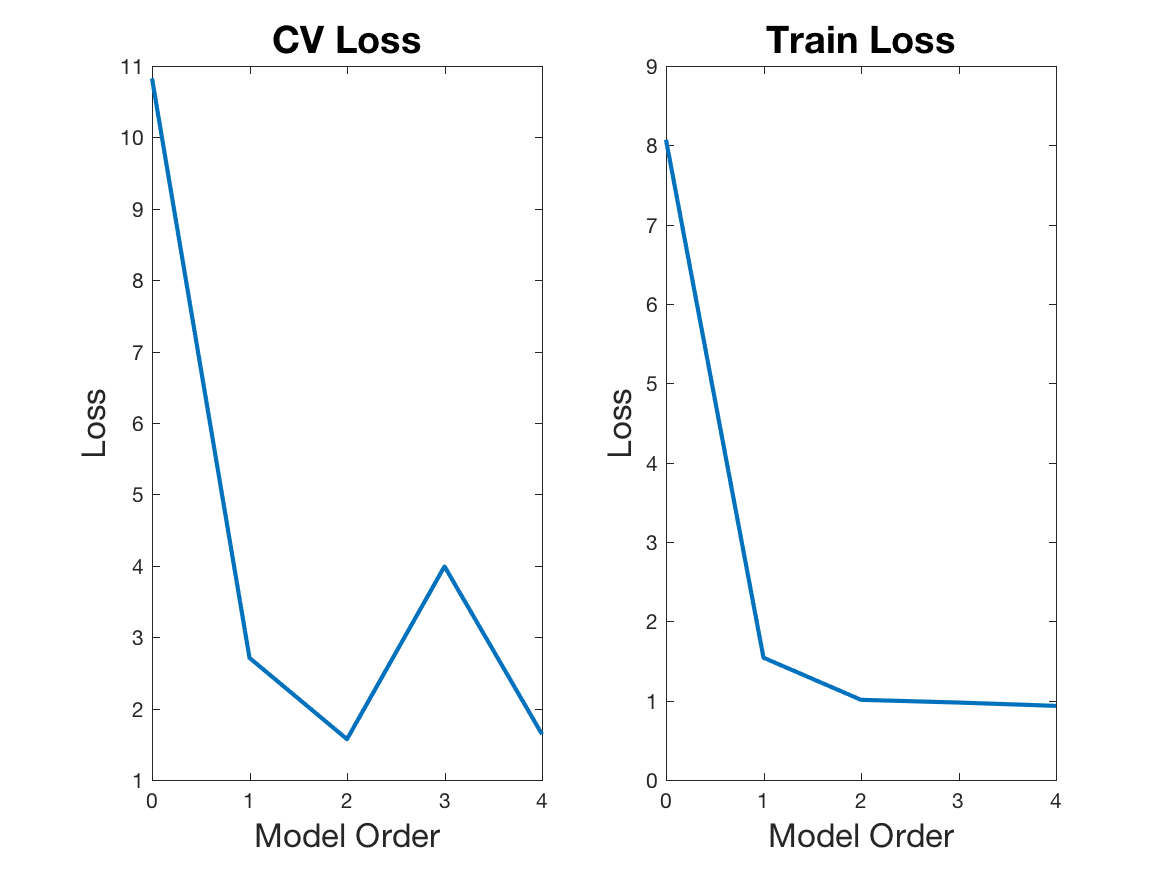
\includegraphics[width=0.8\linewidth]{images/CVLossANDTrainLoss4}
	\caption{Comparison of the CV and Train loss for polynomial models of order \textbf{n}, where \textbf{n} = 0 to 4.}
	\label{fig:CVT4}
\end{figure}

Figure \ref{fig:CVT4} shows if only the CV loss is considered, an order of 2 is slightly better, but if only training loss is considered, an order of 4 is best. Moreover, if both CV and training loss are considered, an order of 4 is best. When both are considered, the minimum mean of the CV and training loss determines the best fit.

\begin{figure}[h!] 
	\centering
	\begin{subfigure}[b]{0.4\textwidth}
		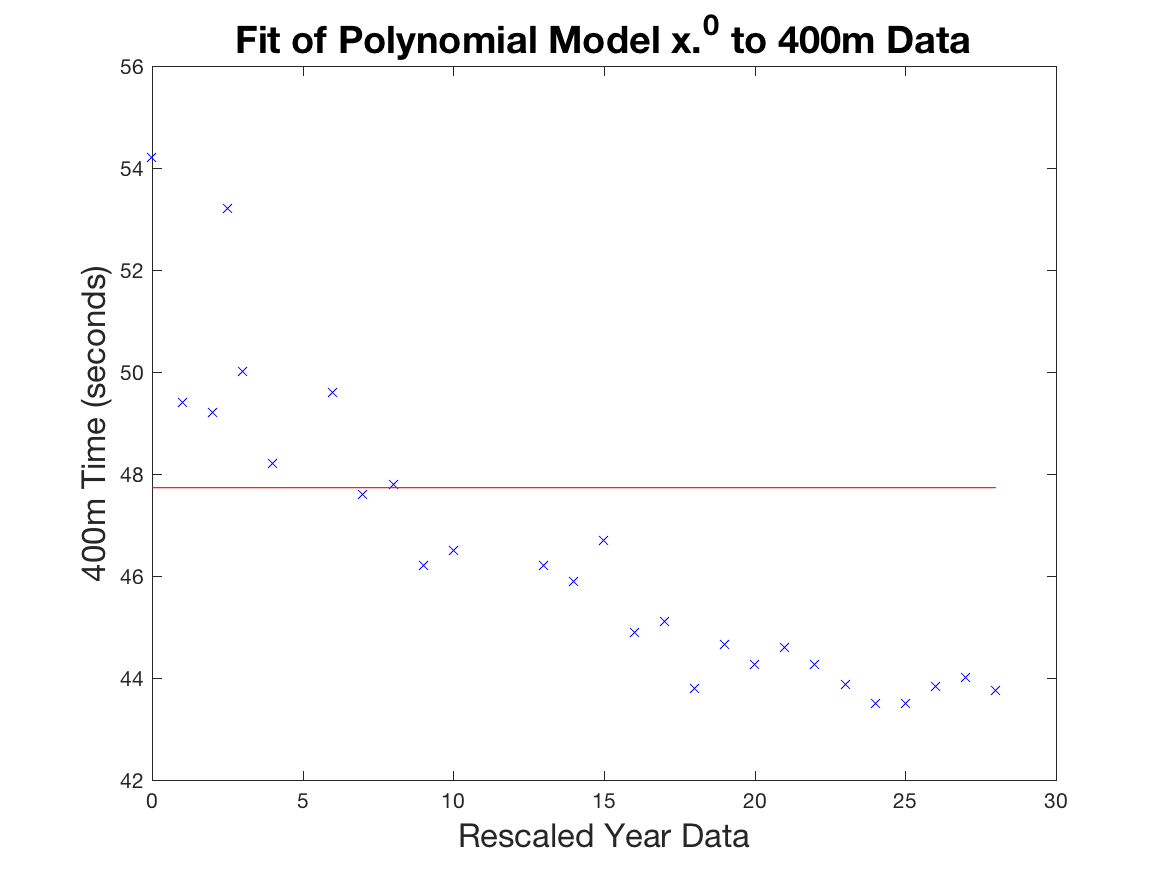
\includegraphics[width=\textwidth]{model0.png}
		\caption{Polynomial model with order \textbf{n} = 0}
		\label{fig:model0}
	\end{subfigure}
	\begin{subfigure}[b]{0.4\textwidth}
		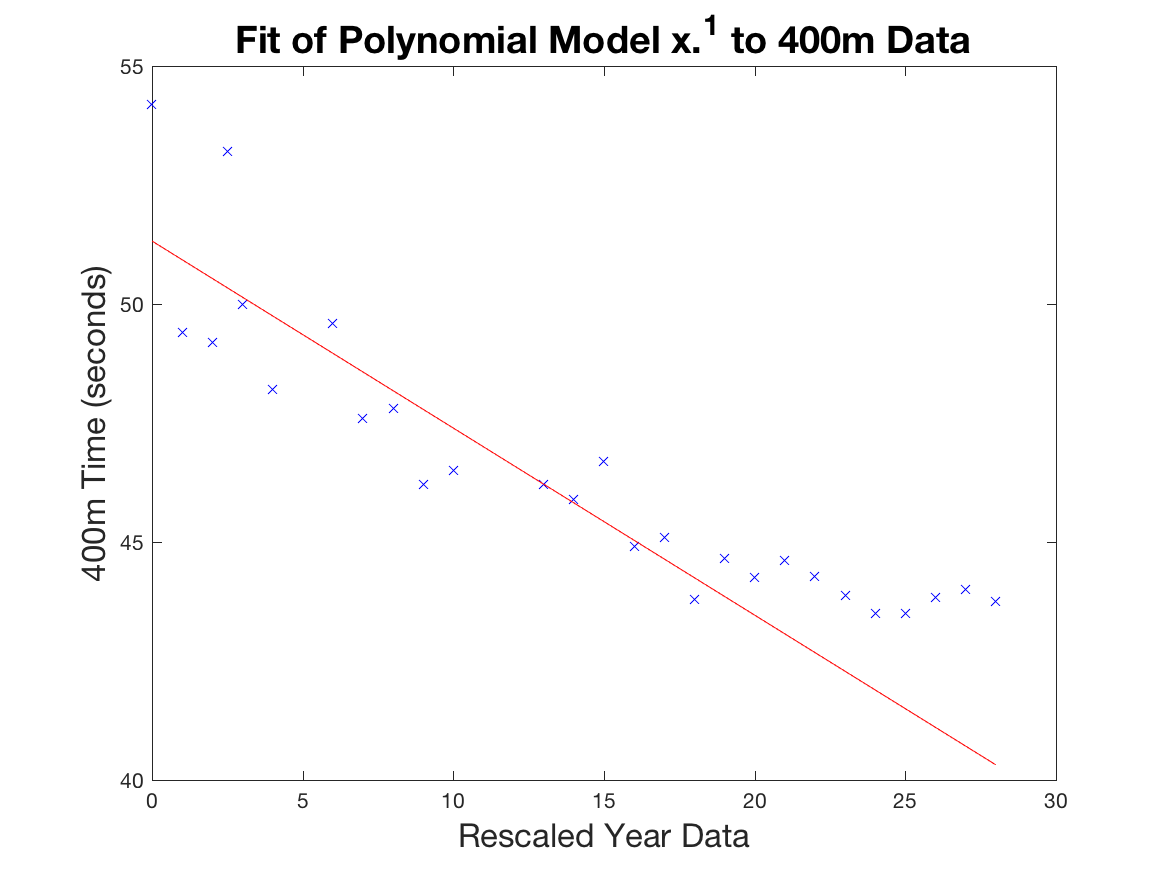
\includegraphics[width=\textwidth]{model1.png}
		\caption{Polynomial model with order \textbf{n} = 1}
		\label{fig:model1}
	\end{subfigure}
	\begin{subfigure}[b]{0.4\textwidth}
		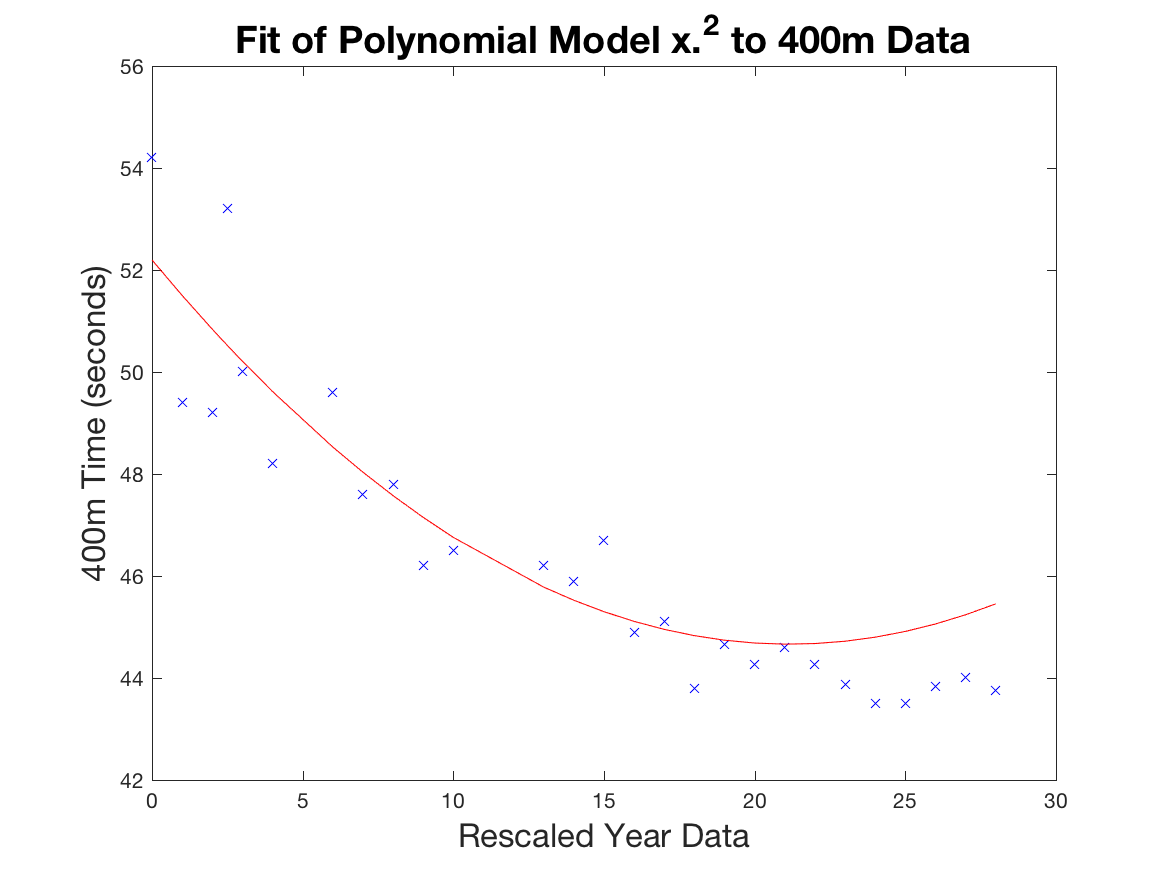
\includegraphics[width=\textwidth]{model2.png}
		\caption{Polynomial model with order \textbf{n} = 2}
		\label{fig:model2}
	\end{subfigure}
	\begin{subfigure}[b]{0.4\textwidth}
		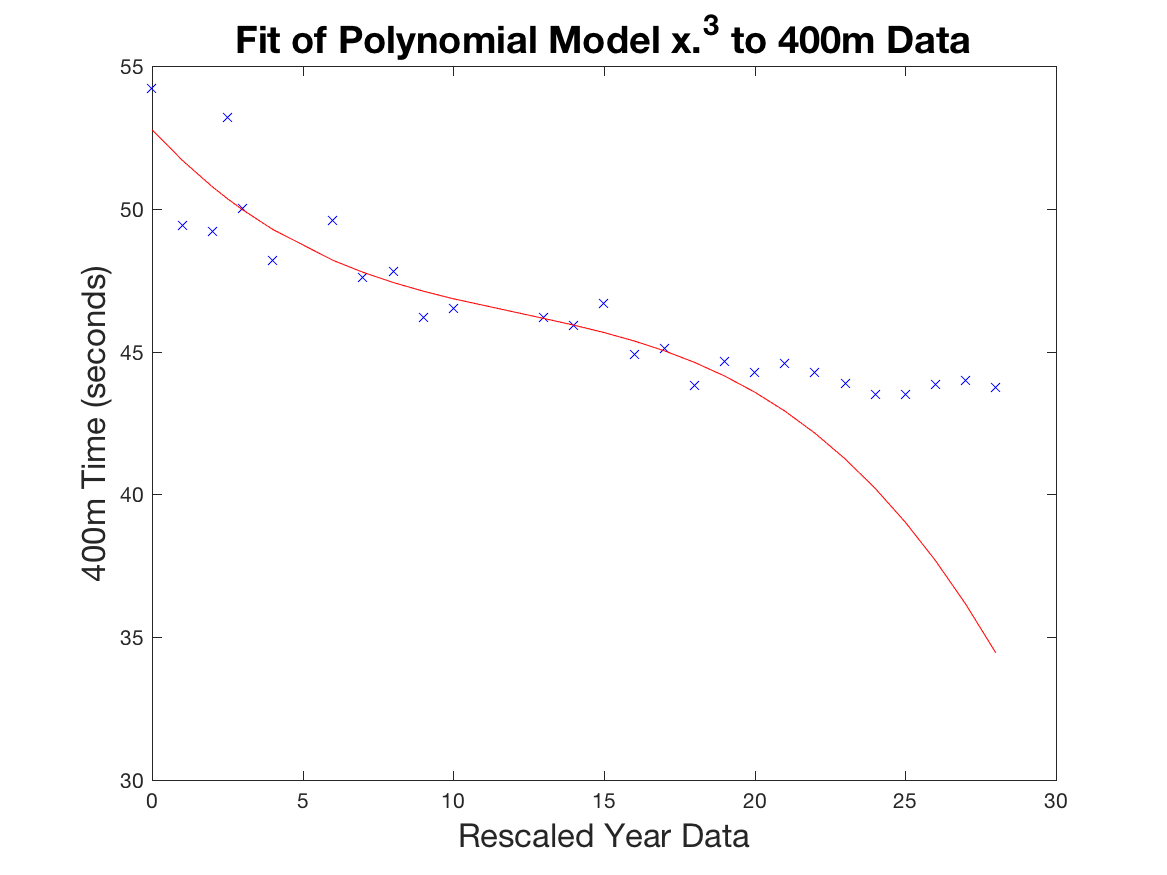
\includegraphics[width=\textwidth]{model3.png}
		\caption{Polynomial model with order \textbf{n} = 3}
		\label{fig:model3}
	\end{subfigure}
	\begin{subfigure}[b]{0.4\textwidth}
		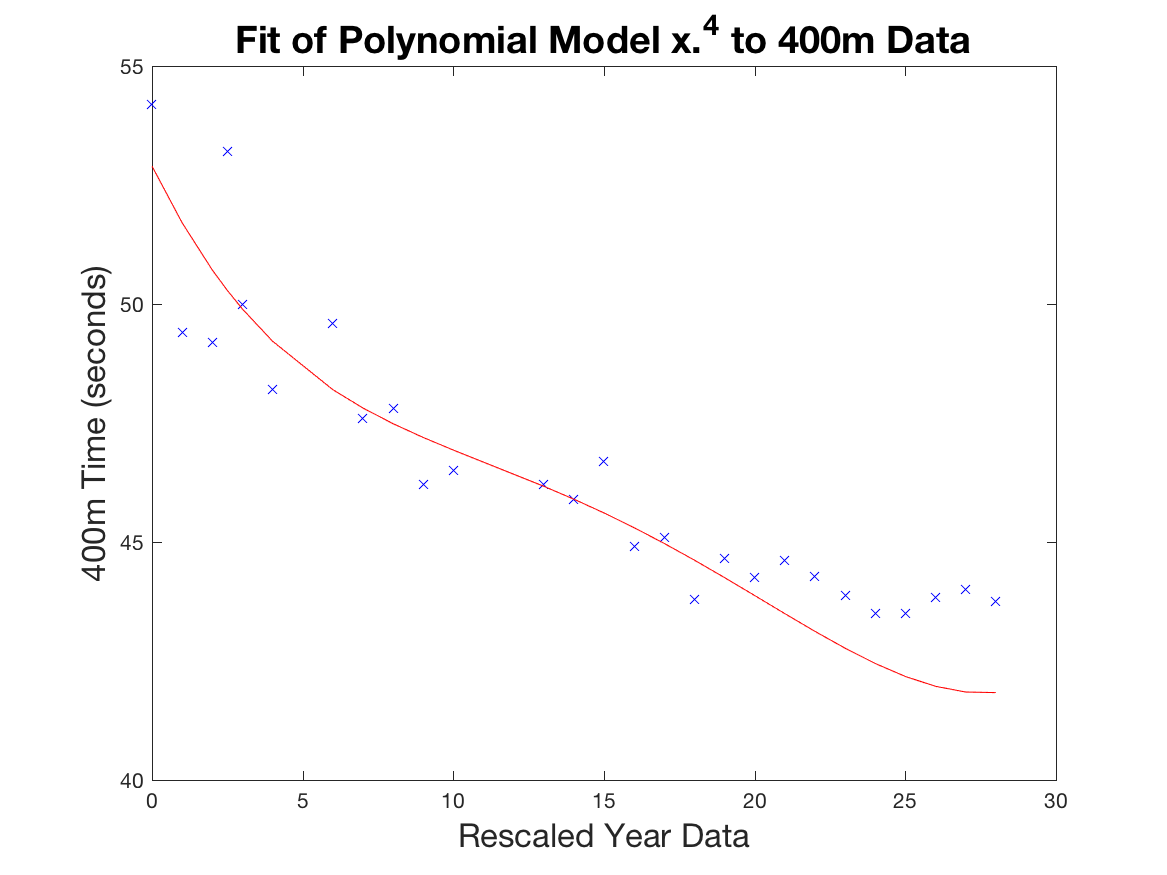
\includegraphics[width=\textwidth]{model4.png}
		\caption{Polynomial model with order \textbf{n} = 4}
		\label{fig:model4}
	\end{subfigure}
	\caption{The original Olympic men's 400m data (blue crosses) with the polynomial models (red) overlaid.}
	\label{men400-1}
\end{figure}

Looking at the Olympics men's 400m data in Figure \ref{men400-1}, the trend is slightly parabolic. This indicates a polynomial function of order 2 is the best fit and Figure \ref{fig:model2} shows how well this model fits. Interestingly, Figure \ref{fig:model4}, shows an order of 4 provides an even closer fit and a more realistic future prediction than an order of 2. In comparison, an order of 2 shows that future predictions would increase in time at an increasing rate. This is highly unlikely given the downward trend of the data.

The remaining models in Figure \ref{men400-1} clearly do not model the data well, where orders 1 and 3 show that a time of 0 will be achieved soon. This is not humanly possibly so the models can be discarded. 

Also, if we do not standardise data, we run into numerical errors when determining the polynomial function of the data with order n. Therefore, it is good practice to standardise data when the regression model contains polynomial terms \cite{WhenIsIt}.

\section{Task 2}
In task 2 we are given the task to find the value of $\lambda$ that gives the 'best' predictive performance on the Olympic men's 100m data using 5-fold cross-validation. In this task, "best" is also defined the same as in \ref{s1}. Refer to Appendix B for the Matlab code used for analysis.

Figure \ref{fig:CVLL4} shows that the best value for $\lambda$ is 0. This is expected for this dataset, as it is linear. Furthermore, a model with a higher order willl fit closer, but increases the risk of over-fitting to the data. This is unlikely to happen with an order of 4 and 27 attributes. If the order was increased to 26 (N - 1), the model would perfectly fit the observed data but this is also an extreme case of over-fitting. To counter this, the lambda value is increased to penalise the over-fitting and generalise the model. A balanced trade-off is often sought between these two variables when dealing with higher order polynomials.

\begin{figure}[h] %example of figure with picture 'h' tells latex to place it 'around' here
	\centering
	\begin{subfigure}[b]{0.45\textwidth}
		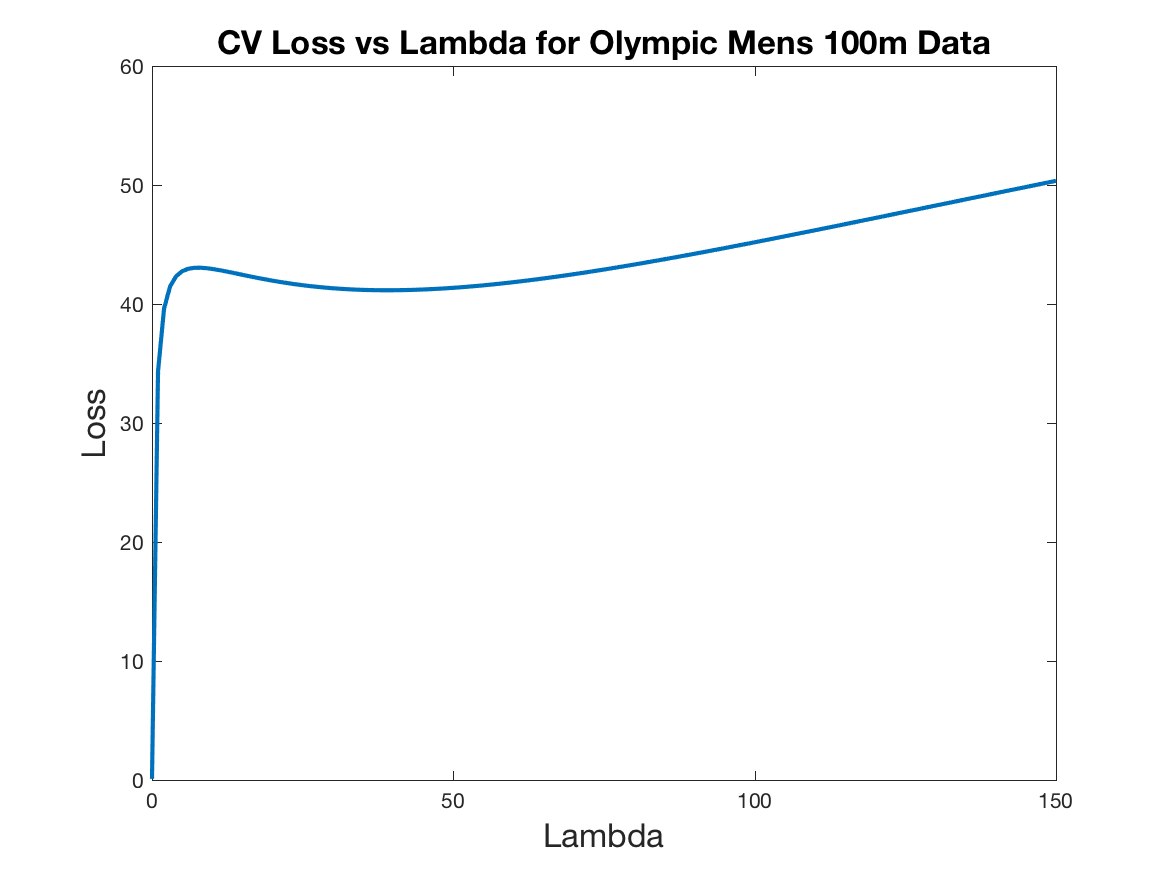
\includegraphics[width=\textwidth]{CVLossvsLambda1.png}
		\caption{Loss of varying lambda values for order 1}
		\label{fig:CVLL1}
	\end{subfigure}
	\begin{subfigure}[b]{0.45\textwidth}
		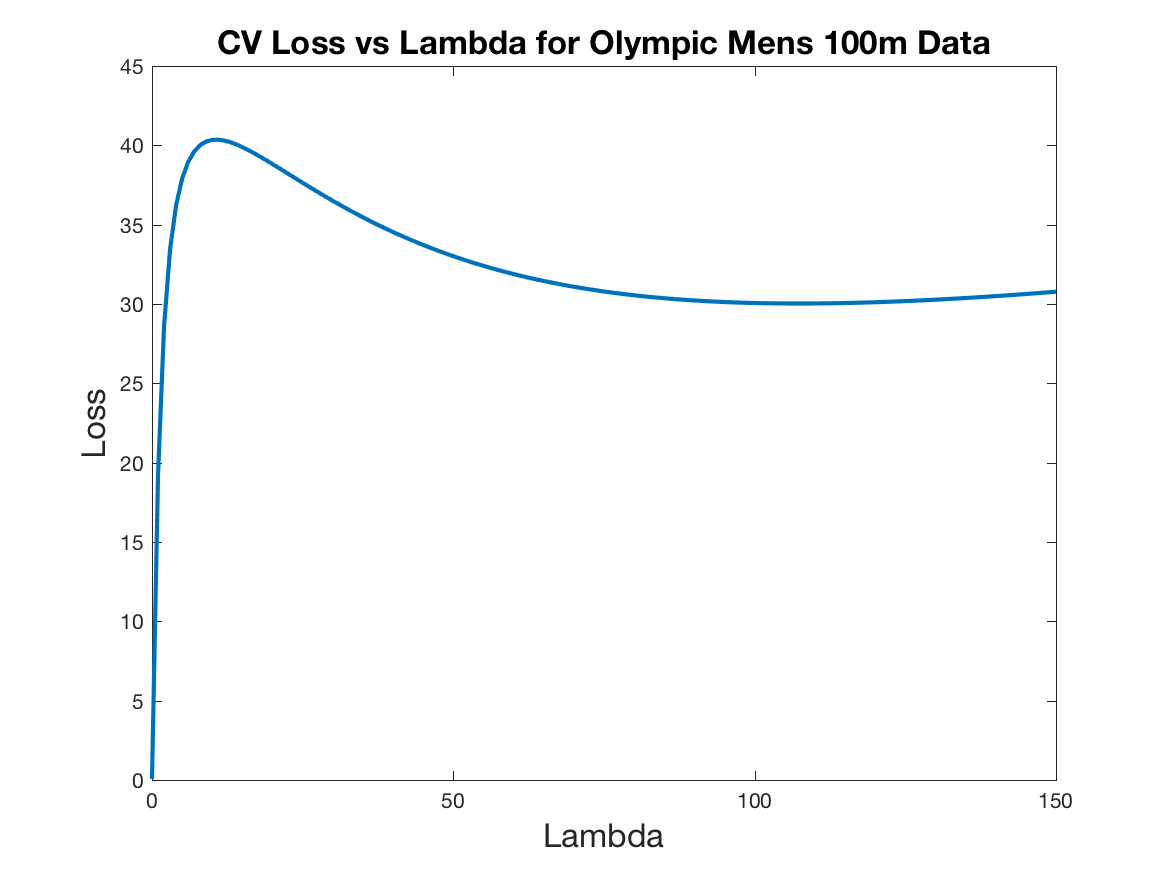
\includegraphics[width=\textwidth]{CVLossvsLambda4.png}
		\caption{Loss of varying lambda values for order 4}
		\label{fig:CVLL4}
	\end{subfigure}
	\caption{The loss vs lambda values for polynomial models with order 1, and 4.}
	\label{fig:LambdaLoss}
\end{figure}

For illustrative purposes, the first 4 values of lambda for both polynomial functions are included in Figures \ref{fig:lambda1} and \ref{fig:lambda2}. These show the increase in model loss as the value of lambda increases.

\begin{figure}[h] 
	\centering
	\begin{subfigure}[b]{0.4\textwidth}
		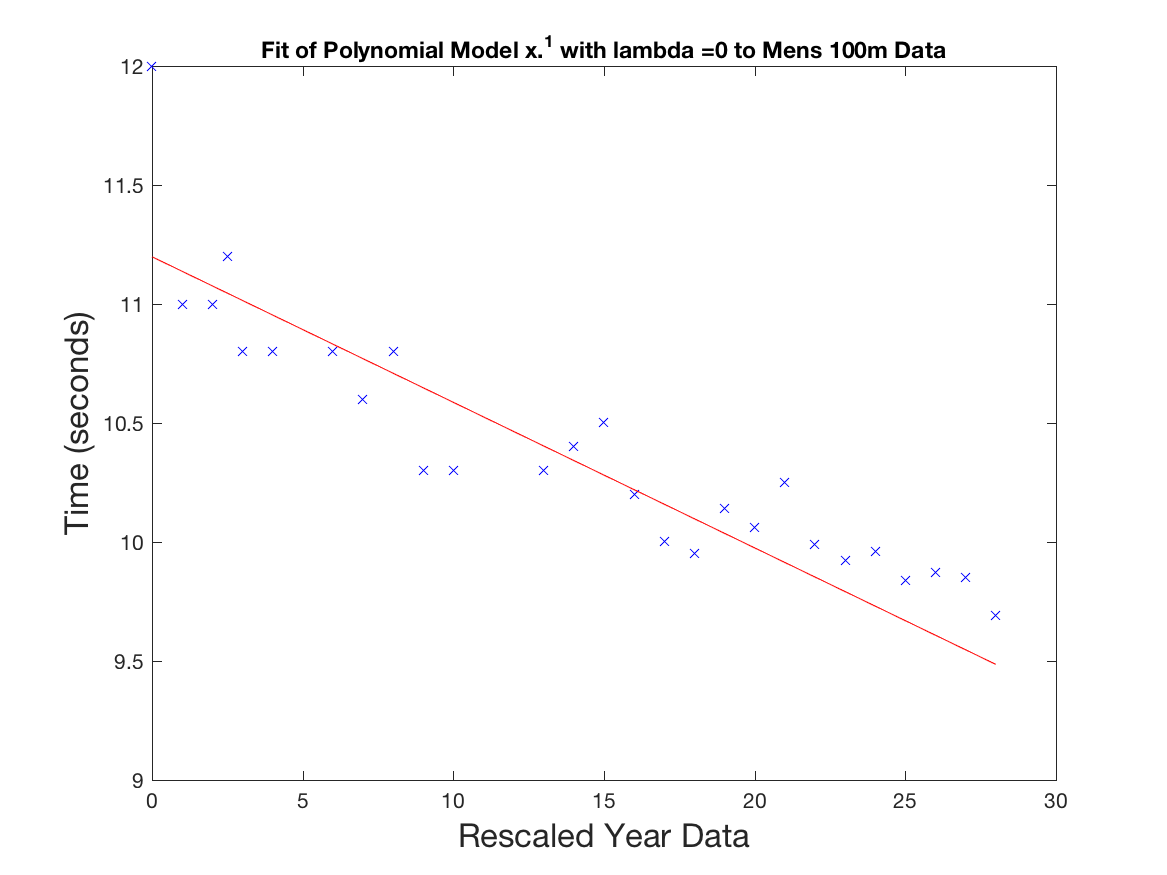
\includegraphics[width=\textwidth]{LambdaModel0_1.png}
		\caption{Lambda = 0}
		\label{fig:model0}
	\end{subfigure}
	\begin{subfigure}[b]{0.4\textwidth}
		\includegraphics[width=\textwidth]{{LambdaModel0.1_1}.png}
		\caption{Lambda = 0.1}
		\label{fig:model1}
	\end{subfigure}
	\quad
	\begin{subfigure}[b]{0.4\textwidth}
		\includegraphics[width=\textwidth]{{LambdaModel0.2_1}.png}
		\caption{Lambda = 0.2}
		\label{fig:model0}
	\end{subfigure}
	\begin{subfigure}[b]{0.4\textwidth}
		\includegraphics[width=\textwidth]{{LambdaModel0.3_1}.png}
		\caption{Lambda = 0.3}
		\label{fig:model1}
	\end{subfigure}
	\caption{Polynomial model with order 1 and varying lambda values.}
	\label{fig:lambda1}
\end{figure}

\begin{figure}[h]
	\centering
	\begin{subfigure}[b]{0.4\textwidth}
		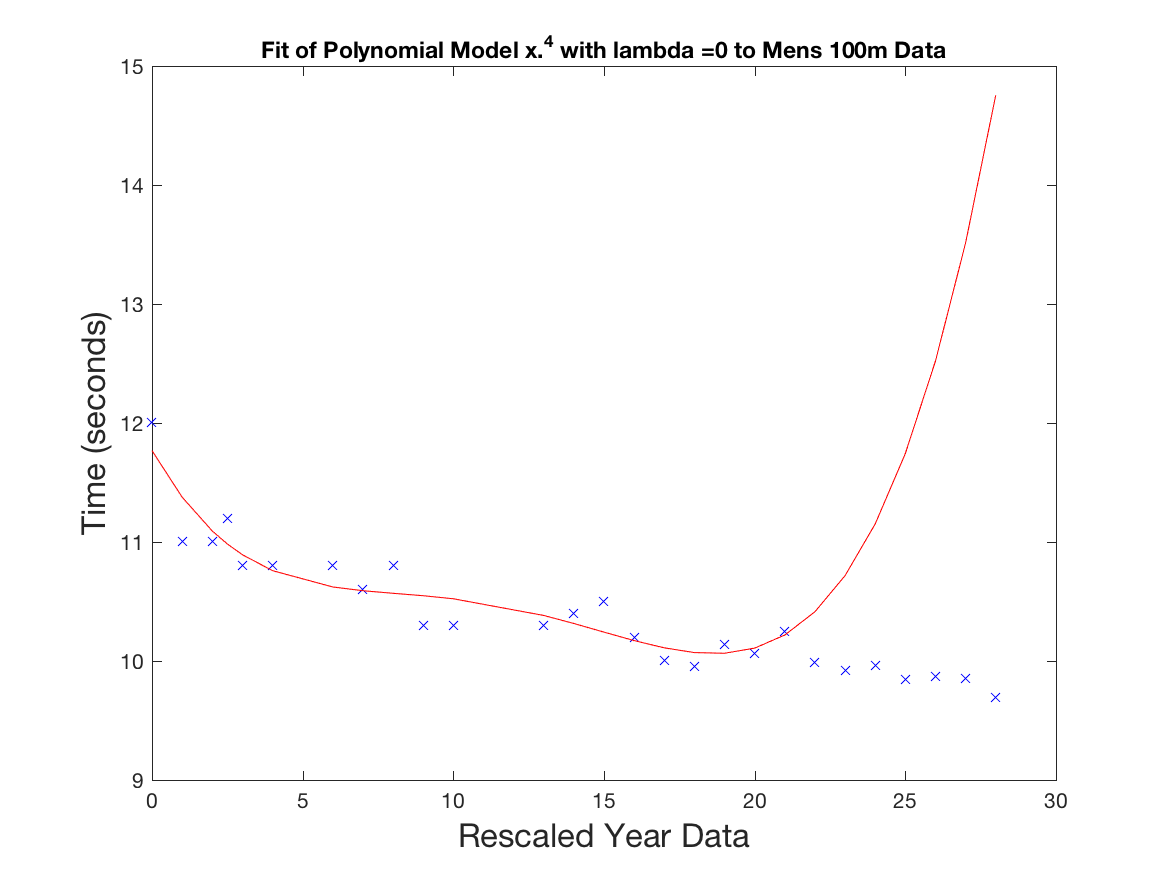
\includegraphics[width=\textwidth]{LambdaModel0_4.png}
		\caption{Lambda = 0}
		\label{fig:model0}
	\end{subfigure}
	\begin{subfigure}[b]{0.4\textwidth}
		\includegraphics[width=\textwidth]{{LambdaModel0.1_4}.png}
		\caption{Lambda = 0.1}
		\label{fig:model1}
	\end{subfigure}
	\quad
	\begin{subfigure}[b]{0.4\textwidth}
		\includegraphics[width=\textwidth]{{LambdaModel0.2_4}.png}
		\caption{Lambda = 0.2}
		\label{fig:model0}
	\end{subfigure}
	\begin{subfigure}[b]{0.4\textwidth}
		\includegraphics[width=\textwidth]{{LambdaModel0.3_4}.png}
		\caption{Lambda = 0.3}
		\label{fig:model1}
	\end{subfigure}
	\caption{Polynomial model with order 4 and varying lambda values.}
	\label{fig:lambda2}
\end{figure}
